% -*- mode: latex; mode: auto-fill -*-

\chapter{Implementation}

This chapter covers the development of the GASP framework, along with
information about how to extend GASP to handle new algorithms.  It
assumes some knowledge of programming in \GAP{}.

\section{Development}

\subsection{First Cut}

When developing the GASP simulation framework, the aim was to have a
simulation framework that could handle as many different spatial
statistical problems as was reasonable while keeping the framework
simple and easy to understand.

It is also desirable that code written for one problem should be
usable in similar problems.

To achieve these goals, I first needed to write a general
representation for configurations of geometric objects.  This led to
the creation of the \texttt{Configuration} and
\texttt{Picture\-Object} types.  The \texttt{Picture\-Object} type
represents the geometric objects that make up the configuration (the
name \texttt{Picture\-Object} was chosen because \texttt{Object} was
already taken by \GAP{}).  Instances of these types cannot be created
directly.  They are \emph{abstract}, so a user must use a derived
type.  For example, the \texttt{Point\-Configuration} and
\texttt{Point} types.

A first approach would be to adopt a simple framework that resembled
the basic Metropolis-Hastings algorithm.  The framework can be written
in terms of the \texttt{Configuration} and \texttt{Picture\-Object}
types.  Parts of the framework that are specific to a particular
algorithm are implemented as calls to functions a user must provide.
This gave us the following basic framework:

Given a configuration to store the state of the simulation, and
user supplied functions \texttt{propose} and \texttt{acceptancecheck}
that implement the algorithm, perform the following steps:

\begin{enumerate}
\item call the user supplied function \texttt{propose} to propose a
change to the configuration.
\item call the user supplied function \texttt{acceptancecheck}
function to calculate the probability of accepting the proposition.
\item make a random decision whether to to accept with the probability
calculated in the previous step:
\begin{itemize}
\item if accepted, make the change to the configuration
\item if rejected, do nothing
\end{itemize}
\item repeat from first step
\end{enumerate}

At this point, the return value of the function \texttt{propose} is
limited to proposing to create a new object or delete an existing
object.  These are represented by lists of length 2 -- the first
element being a constant representing the type of change, and the
second being the object that we are adding or deleting.

This simple framework exhibits a number of limitations.  For instance,
the \texttt{propose} and \texttt{acceptancecheck} functions are
implemented in terms of the particular \texttt{Configuration} used in
the algorithm.  This means that those functions would need to be
modified if we wanted to run the same algorithm with a different
\texttt{Configuration}.  This framework also limited the allowable
propositions to adding and removing points.


\subsection{Virtualisation}

In order to get around the first problem, I virtualised most of the
actions that are performed on \texttt{Configuration}s and
\texttt{Picture\-Object}s.  This means that rather than accessing the
configuration directly, the algorithm calls functions provided with
the configuration implementation that perform the actions.  We achieve
this through a number of \GAP{} operations.  While it simplifies the
job of the person implementing new algorithms, this change adds the
burden of implementing a number of operations (such as calculating the
distance between two objects, counting objects in a configuration,
checking for objects close to a particular object, etc).  As I expect
that there will be many more algorithms implemented for the framework
than configuration types, the tradeoff seems appropriate.

This made it possible to implement new algorithms in such
a way they could be used with different types of configurations
without modification, which also gives more flexibility to change how
various parts of the framework are implemented.

The list of operations for use when writing proposal or acceptance
check functions is covered in Section \ref{sect:new-algorithms}


\subsection{Change Objects and the Change Log}

In order to lift the restriction on the allowed types of change that
may be made to configurations, rather than using a two element list, I
created a new type called a \texttt{Change} object.  The idea behind
\texttt{Change} objects in the simulation framework is very similar to
the way undo capabilities are implemented in many applications.  These
objects package up all the information about how to \emph{apply}
themselves to the configuration, and how to \emph{revert} any changes
they made to the configuration.

We could now modify the simulation framework to look like:

\begin{enumerate}
\item call the user defined \texttt{propose} function, which returns a
\texttt{Change} object representing the proposed change to the
configuration.
\item apply the \texttt{Change} object to the configuration.
\item call the \texttt{acceptancecheck} function to calculate the
probability of accepting the change.
\item make a random decision whether to accept the change with the
calculated probability.  If the proposal is rejected, revert the
change.
\item go to step 1 and repeat.
\end{enumerate}

All information about an iteration is written to a log file.  This
includes the change that was proposed, the calculated probability and
whether the proposal was accepted.  More information about the log
file is found in Section \ref{sect:log-file}


%\subsection{Continuation Checks}
%
%\emph{XXXX - short description of continuation check part of framework}


\section{Implementing New Algorithms}\label{sect:new-algorithms}

This section covers the parts of the GASP application programming
interface required to write new proposal and acceptance check
functions.  The user will need to have a basic knowledge of the \GAP{}
syntax along with knowledge of the following programming interfaces.
The \GAP{} Tutorial \cite{gap-tut} is a good introduction to using the
\GAP{} language.  This information is necessary for simulating
processes that are not covered by the existing algorithms distributed
with GASP.

More specifically, the user will need to know how to write functions
and use simple programming structures.

\subsection{Configuration Operations}

In order to implement the proposal and acceptance check functions, it
will be necessary to make calculations based on a given configuration.
A number of operations are provided to access the configuration so
that the algorithms the user implements are not dependent on a
particular configuration implementation.

These operations have to be implemented for each configuration type.
Here is a list of the operations most useful when implementing
proposal and acceptance checking functions:

\subsubsection{ConfigWindowArea}

The \texttt{ConfigWindowArea} operation can be used to calculate
simulation region.  This is used in a number of problems when
calculating acceptance probabilities:
\begin{lstlisting}{}
area := ConfigWindowArea(config);
\end{lstlisting}

\noindent Here, \texttt{config} is a \texttt{Configuration} object.

\subsubsection{RandomNewObject}

In the proposal function for a particular algorithm, it will usually
be necessary to create new objects for the configuration.  The
operation \texttt{Random\-New\-Object} can be used to do this:
\begin{lstlisting}{}
obj := RandomNewObject(config);
\end{lstlisting}

\subsubsection{ChooseRandomObject}

\texttt{ChooseRandomObject} picks a random existing object from a
given configuration.  This might be useful in a proposal function.
\begin{lstlisting}{}
obj := ChooseRandomObject(config);
\end{lstlisting}

\subsubsection{CountObjects}

The operation \texttt{CountObjects} counts the total number of objects
in a given configuration. It may be useful when calculating the
acceptance probability.
\begin{lstlisting}{}
num := CountObjects(config);
\end{lstlisting}

\subsubsection{CountObjectsWithMark}

For algorithms where we work with objects with marks attached (marks
were defined in Section \ref{sect:glossary}), it may be useful to
count the objects that have a particular mark set.  This is done with
the operation \texttt{CountObjectsWithMark}:
\begin{lstlisting}{}
num := CountObjectsWithMark(config, markname);
\end{lstlisting}

\noindent The argument \emph{markname} is the name of the mark that
must be set on the objects that are being counted.  For more
information on the marks interfaces, see Section
\ref{sect:user-desc-marks}.

\subsubsection{GetObjectsWithMark}

Some algorithms may require a list of all the objects that have a
particular mark.  This can be achieved with the operation
\texttt{GetObjectsWithMark}:
\begin{lstlisting}{}
object_list := GetObjectsWithMark(config, markname);
\end{lstlisting}

\noindent The argument \emph{markname} for this function has the same
meaning as the one in the \texttt{CountObjectsWithMark} operation.

\subsubsection{CloseObjects}

For some algorithms we require some information about how many objects
in the configuration are within a certain distance of a particular
object.  The \texttt{CloseObjects} operation is used to calculate this:
\begin{lstlisting}{}
num := CloseObjects(config, object, rad);
\end{lstlisting}

\noindent This is the function is basically the same as the function
$s(\mathbf{x}, y)$ used in the calculation of the acceptance
probability of the Strauss Process.  As with $s(\mathbf{x}, y)$, if
\emph{object} is already part of the configuration, then it will not
be included in the count.

\subsubsection{CloseObjectsWithMark}

For algorithms that involve marks, it may be necessary to perform a
count as in \texttt{CountObjects}, but only counting objects that have
a particular mark set.  For this, the \texttt{CountObjectsWithMark}
operation can be used:

\begin{lstlisting}{}
num := CloseObjectsWithMark(config, object, rad,
                            markname);
\end{lstlisting}

\subsection{The Marks Interfaces}\label{sect:user-desc-marks}

For algorithms that involve marks, the user may need to know about the
marks interfaces for objects in the GASP package.  When creating new
objects, it is necessary to set the appropriate marks on the object.
When writing the acceptance check function, it may be necessary to
check for a mark on an object.

The marks interfaces in GASP work on a set of boolean marks associated
with an object.  For multi-valued marks, it must be implemented as a
set boolean marks for each possible value.  The algorithm should make
sure that it does not set conflicting marks on an object.

The marks for an object are manipulated with three different
operations:

\begin{description}
\item[\texttt{AddMark(object, markname)}] sets the mark
\emph{markname} on the given object.
\item[\texttt{DelMark(object, markname)}] unsets the mark
\emph{markname} on the given object.
\item[\texttt{HasMark(object, markname)}] returns true if the mark
\emph{markname} is set on the given object, and returns false
otherwise.
\end{description}

\subsection{The Proposal Function}\label{sect:proposal-function-impl}

The proposal function for an algorithm decides on a change to propose
based on the current state of the configuration.  The prototype for
all proposal functions is:
\begin{lstlisting}{}
change := propose(config);
\end{lstlisting}

\noindent The return value is a change object representing the change
that is proposed.  These \emph{change objects} contain all the
information required to move to the next state.  There are a number of
predefined change objects that can be used in the algorithm.  It is a
little more involved to implement new change object types.

\subsubsection{AddObjectChange}

The \texttt{AddObjectChange} type is used when proposing the addition
of a new object.  The user can create such a change with the following
syntax:

\begin{lstlisting}{}
change := AddObjectChange(object);
\end{lstlisting}

\noindent The object inside the change can be accessed with
\texttt{change!.obj} if needed later.


\subsubsection{DelObjectChange}

Removing an object is achieved with the \texttt{DelObjectChange}
type.  This type is created with the following function call:

\begin{lstlisting}{}
change := DelObjectChange(object);
\end{lstlisting}

\noindent Again, access to the object that is being removed is
available as \texttt{change!.obj}.


\subsubsection{ReplaceObjectChange}

In the case of moving an object, a new object in the new position
should be be created and a change that \emph{replaces} the old object
with the new one should be used.  This type of change can be created
with the following syntax:

\begin{lstlisting}{}
change := ReplaceObjectChange(addobj, delobj);
\end{lstlisting}

\noindent The two objects in the change can be accessed as
\texttt{change!.addobj} and \texttt{change!.delobj} if needed.

\subsubsection{ReplaceMultipleObjectsChange}

If the algorithm requires replacing one set of objects with another in the
configuration, then \texttt{ReplaceMultipleObjectsChange} can be used.

\begin{lstlisting}{}
change := ReplaceMultipleObjectsChange(addobjs,delobjs);
\end{lstlisting}

\noindent The two arguments to this function are lists of objects that
are to be replaced.

\subsection{The Acceptance Check Function}

The acceptance check function for the algorithm calculates the
probability of accepting the proposed state.  The prototype for all
acceptance check functions is:

\begin{lstlisting}{}
probability := acceptancecheck(config, change);
\end{lstlisting}

\noindent When the acceptance check function is called, the
configuration will already be in the proposed state.  The change that
was performed is passed as an argument in case that is needed when
calculating the acceptance probability.

For some algorithms, it may be necessary to check what \emph{type} of
change was proposed.  For each of the change objects, there is a
boolean function to check for that type.  These are just the name of
the change type with `Is' prepended.  There are
\texttt{IsAddObjectChange}, \texttt{IsDelObjectChange},
\texttt{IsReplaceObjectChange} and
\texttt{IsReplaceMultipleObjectsChange}.

\subsection{An Example}\label{sect:red-black-example}

To put this into practice, we look at an example of implementing an
algorithm from scratch with GASP.  We reimplement the Widom-Rowlinson
point process, which does not fit as neatly into the simulation
framework as some other algorithms.

For this process, we implement the bulk of the algorithm in the
proposal function.  The proposal function performs one phase of the
algorithm (that is, remove all points of a particular colour, and add
new points of that colour).  The acceptance check function always
returns a probability of 1 to accept the change.  We also keep some
extra information in the configuration to keep track of whether we are
supposed to be adding red or black points in the next iteration.

For this example, we use a 300 by 300 configuration, a minimum
distance of 15 and 100 and 120 as means of the Poisson distributions
for the number of red and black points respectively.

\lstset{labelstyle=\tiny,labelstep=4}
\begin{lstlisting}{}
# create a configuration object
config := PointConfiguration(0,0,300,300);
# the first iteration will add black points
config!.isRedIter := false;

rad := 15;
# set up Poisson random number generators
red_rnd := CreatePoissonRNG(100);
black_rnd := CreatePoissonRNG(120);

# define the proposal function for the algorithm
propose := function(config)
    local del, add, obj, num, i, RandRat;

    # are we adding red points during this iteration?
    if config!.isRedIter then
        # we want to replace all existing red points
        del := GetObjectsWithMark(config, "red");
        add := [];
        num := red_rnd();  # number of points to add
        for i in [ 1 .. num ] do
            obj := RandomNewObject(config);
            AddMark(obj, "red");
            # add the object if it is far enough away
            # from the black points
            if CloseObjectsWithMark(config, obj, rad,
                                    "black") = 0 then
                Append(add, [ obj ]);
            fi;
        od;
    else
        # we want to replace all existing black points
        del := GetObjectsWithMark(config, "black");
        add := [];
        num := black_rnd();  # number of points to add
        for i in [ 1 .. num ] do
            obj := RandomNewObject(config);
            AddMark(obj, "black");
            # add the object if it is far enough away
            # from the red points
            if CloseObjectsWithMark(config, obj, rad,
                                    "red") = 0 then
                Append(add, [ obj ]);
            fi;
        od;
    fi;
    config!.isRedIter := not config!.isRedIter;
    return ReplaceMultipleObjectsChange(add, del);
end;

# now the acceptance check function
acceptance_check := function(config, change)
    return 1;
end;

# finally, start up the graphical user interface
GUISimulate(config, "Red-Black", 300, 300,
            propose, acceptance_check);
\end{lstlisting}

\noindent This example will bring up the GUI where the user can run
the simulation.  On lines 8 and 9, we create Poisson random number
generators used to calculate the number of points in the simulation.
The rest of the example is fairly straight forward.  The simulation
should look something like Figure \ref{fig:red-black-output}.

\begin{figure}[hbt]
\centering
\framebox{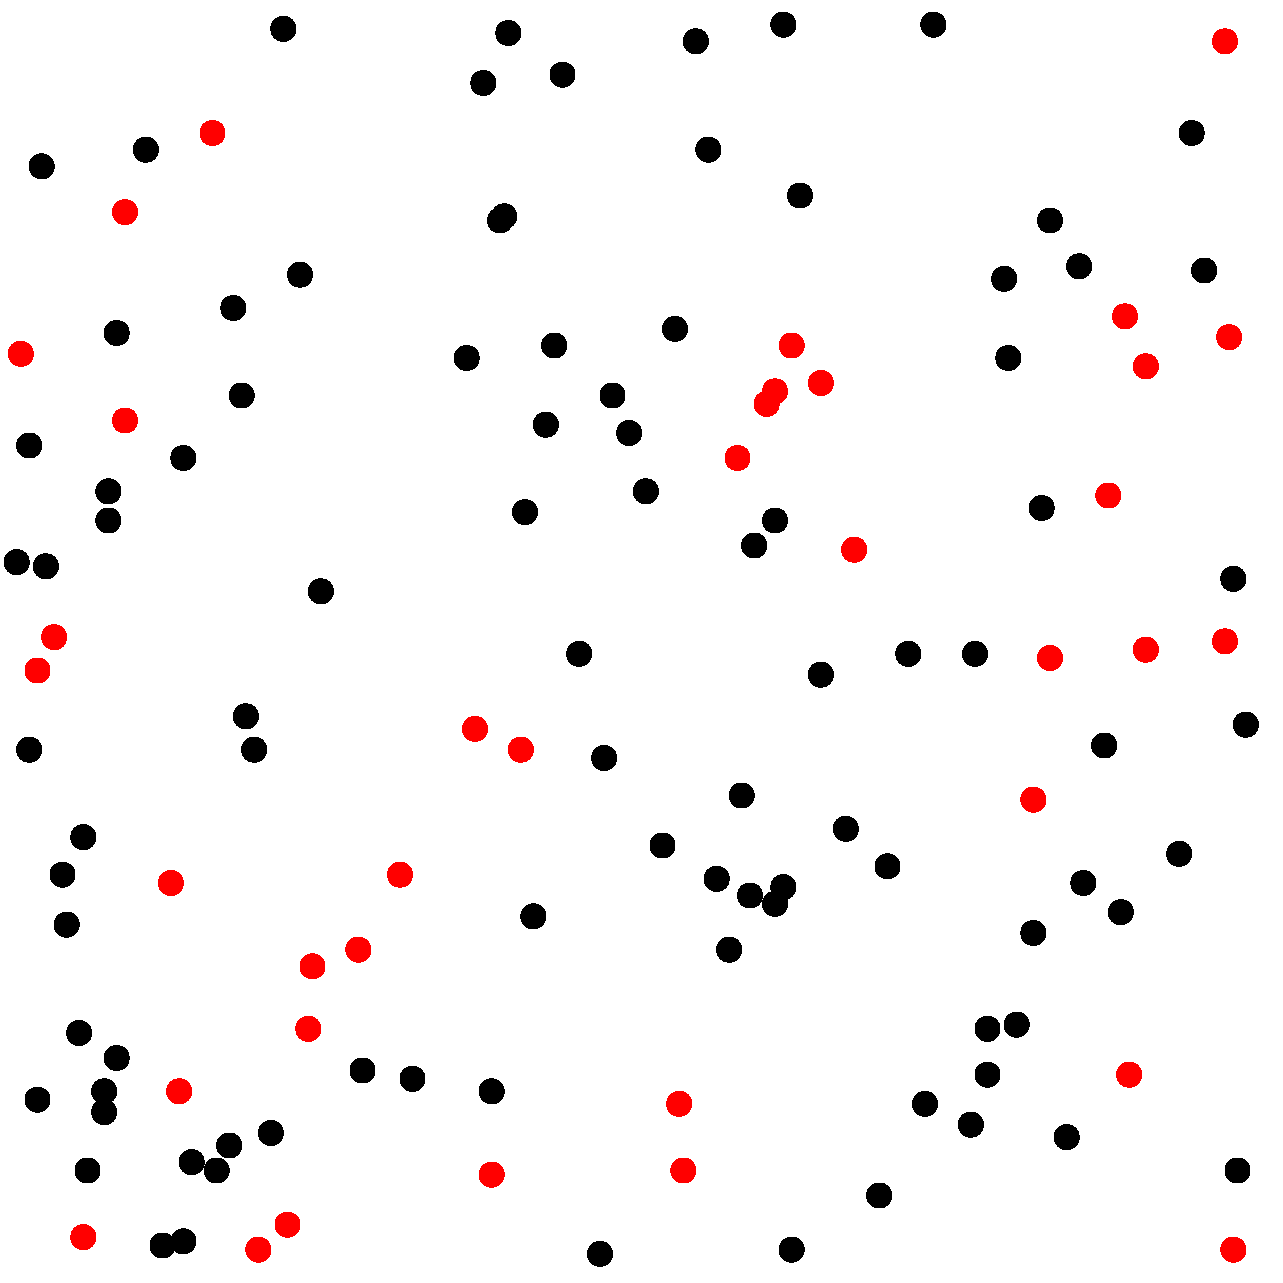
\includegraphics[width=4in]{red-black}}
\caption{Red-Black Point Process}
\label{fig:red-black-output}
\end{figure}

This particular algorithm can also be used through the existing
\texttt{Create\-RedBlack\-Propose}, and the \texttt{CreateFixedCheck} with
a probability of $1$.


% \emph{XXXX - should we put this section into this chapter rather than
%previous one?}

\section{Creating New Configuration Types}

For some problems, the supplied configuration types are not
sufficient.  Either the type of objects that make up the state are not
covered by the provided configuration types or the existing
configurations are not efficient enough.

As an example of the second case, if we had an algorithm that
performed a lot of checks to count the objects close to a particular
object, then it may be appropriate to use a different configuration
type that was more optimised for that sort of operation.  Such an
optimisation would be to sort the objects into bins according to where
they are located in the plane.  Now to find all objects within a given
radius $r$ of a particular object $y$, we only have to check the bins that
are within a radius $r$ of the bin that contains $y$.  While this
internal representation for the configuration speeds up these distance
checking operations, it slows down other operations such as counting
all objects in the configuration.

The creation of new configuration types requires knowledge of the
\GAP{} object model.  This is covered in the \emph{Programming in
\GAP{} 4} manual \cite{gap-prg} that is distributed with \GAP{}.

New configuration types must be derived from the abstract object
category \texttt{IsConfiguration}.  If a new object type is required,
it must derive from \texttt{IsPicture\-Object}.

Any new configuration must implement all the operations listed in the
previous section.  In addition to those operations, the new configuration
must implement a number of operations that are used to implement
various parts of GASP.  The extra operations are:
\begin{description}
\item[\texttt{AddObject}] - this operation is used to add an object to
the configuration.  It is not designed to be called by algorithms
directly.  Instead, it is used to implement change objects that add
objects to the configuration.  The prototype for this operation is:
\begin{lstlisting}{}
AddObject(config, object);
\end{lstlisting}
\item[\texttt{DelObject}] - this operation is used to delete an object
to the configuration.  As with \texttt{AddObject}, it is not designed
to be called by algorithms directly.  The prototype for this operation
is:
\begin{lstlisting}{}
DelObject(config, object);
\end{lstlisting}
\item[\texttt{DrawConfiguration}] - this operation is used to draw the
configuration of objects to a graphic sheet.  This will generally be
implemented by calling the \texttt{DrawObject} method on each object
in the configuration.  The prototype is:
\begin{lstlisting}{}
DrawConfiguration(config, graphicsheet);
\end{lstlisting}
\end{description}

The objects that make up the configuration need only implement a few
operations.  The two required operations are:
\begin{description}
\item[\texttt{SquareDistance}] - this operation calculates the square
of the distance between two objects.  The prototype for
\texttt{Square\-Distance} is:
\begin{lstlisting}{}
distance := SquareDistance(object, otherobject);
\end{lstlisting}
\item[\texttt{DrawObject}] - this operation is responsible for drawing
the object to an \XGAP{} graphic sheet.  The prototype for
\texttt{Draw\-Object} is:
\begin{lstlisting}{}
DrawObject(object, graphicsheet);
\end{lstlisting}
\end{description}

Provided that the new object type is implemented as an objectified
record, then the marks operations need not be implemented.  Otherwise,
those interfaces must be reimplemented for the object type.

For more information on implementing new configurations, see the
implementation of the \texttt{Point\-Configuration} type in the GASP
package.

\section{Change Objects}

Change objects are used in the GASP framework to represent all changes
made to configuration objects.  GASP comes with a number of useful
change object types, which were described in Section
\ref{sect:proposal-function-impl}.

New change objects must derive from the abstract category
\texttt{IsChange}.  A change object contains all the information that
is required to apply the change to the configuration, or to revert it
once applied.  These two actions on the configuration are handled by
the following two operations:

\begin{lstlisting}{}
ApplyChange(change, config);
RevertChange(change, config);
\end{lstlisting}

\noindent These operations must be implemented for each new change
type.  Usually a change object is implemented in terms of the
\texttt{AddObject} and \texttt{DelObject} operations of the
\texttt{Configuration} type, so that it may be used with more than one
configuration type.

It is also desirable that the new change object type implement the
standard \GAP{} operation \texttt{PrintObj}, which is used to print a
representation of the object to a file.  This operation will be called
when writing the type of change to the log file.  For this reason, it
is required that \texttt{PrintObj} write the code necessary to
recreate the object.  If this operation is not implemented correctly,
the usefulness of the log file is greatly reduced.

\subsection{The Log File}\label{sect:log-file}

Provided that the user turned on logging, all changes to the
configuration are written to a log file.  The lines in the log file
look similar to:

\begin{indent}
\texttt{[ }\emph{change}\texttt{, }\emph{acceptprob}\texttt{,
}\emph{accept}\texttt{ ]}
\end{indent}

\noindent Here, \emph{acceptprob} is the calculated probability of
accepting the change and \emph{accept} is a boolean representing
whether or not the change was actually accepted and applied.

The log file contains all the information required to replay the
simulation to recreate the final state of the simulation.  In fact, it
is possible to replay the simulation up to any point by using the
log.  This could be used to play back the simulation at a faster rate.

The log is also a useful source of statistics about the run of the
simulation.  For instance, we can look for patterns in the types of
changes that are proposed and the acceptance rates.  Some interesting
information the log could provide are:

\begin{itemize}
\item states for which proposals are given very low acceptance
probability.
\item lengths of runs of acceptances or rejections.
\item changes in the acceptance probability over time.
\end{itemize}

I have not completed the framework to used to parse the log file for
post simulation analysis.  When the log parsing framework is complete,
it will be added to the GASP package.  However, parsing the log is
very simple, as each line is a valid \GAP{} expression.  So it is
possible to read the log before the log parsing framework is complete.
